% target: 8-10ish pages
\chapter{Methodology}
The goal of this chapter is to give an overview of the general evaluation setup and methodology behind our approach, as this ties together the relation between our approach and its evaluation.
The approach we present is the result of several iterations of design and experimentation, as one would expect in the field of distributed systems engineering.

First, we give an introduction to FaaS-Sim, the serverless edge computing simulator we use and extend and the devices included in the simulation.\\
Next we dive into more detail about the simulation setup by describing the serverless functions deployed, along with their performance characteristics.
In this section we also describe how the network simulation part of the simulator is implemented and how the network topologies used in the evaluations are structured.\\
From there we describe how empirical measurements and experiments are integrated in FaaS-Sim to improve its representation of real serverless systems.\\
Lastly, we conclude this chapter by outlining the metrics and \glspl{kpi} captured in our simulation experiments.

\section{Simulating Serverless Edge Computing Systems}
We choose FaaS-Sim\cite{faas-sim-github} as our simulation framework.
FaaS-Sim is is a state of the art serverless computing simulation built on SimPy, %todo cite simpy
a discrete even simulation tool.
From an architectural basis, FaaS-Sim is built to mimic a serverless framework similar to OpenFaaS.
FaaS-Sim is built on top of a simulated Kubernetes infrastructure, meaning that it too has the notion of containers, container images, resource requirements, scaling, and scheduling.
Because FaaS-Sim is built with evaluating serverless edge computing in mind, it also includes support for representing a wide array of node hardware with heterogeneous capabilities and performance.
\begin{table}[]
\begin{tabular}{lcccc}
\hline
\textbf{Bin}        & \textbf{LOW}  & \textbf{MED} & \textbf{HIGH} & \textbf{VERY HIGH} \\ \hline
CPU Cores (logical) & 1 - 2         & 4 - 8        & 16 - 32       & \textgreater 32    \\
Memory              & 1 to 2        & 4 - 8        & 9 - 32        & \textgreater 32    \\
CPU Frequency (GHz) & \textless 1.5 & 1.6 - 2.2    & \textless 3.5 & \textgreater 3.5   \\ \hline
\end{tabular}
\caption{Resource binning used for performance categorization and prediction with Ether devices by Raith, Rausch and Dustdar\cite{philipp-da}}
\label{tab:ether_bins}
\end{table}

\begin{table}[]
\begin{tabular}{lrrrrr}
\hline
\textbf{\begin{tabular}[c]{@{}l@{}}Device\\ Name\end{tabular}} & \textbf{\begin{tabular}[c]{@{}r@{}}CPU\\ Arch\end{tabular}} & \textbf{\begin{tabular}[c]{@{}r@{}}CPU\\ Cores\end{tabular}} & \textbf{\begin{tabular}[c]{@{}r@{}}CPU\\ Freq\end{tabular}} & \textbf{\begin{tabular}[c]{@{}r@{}}Memory\\ GiB\end{tabular}} & \textbf{GPU/AI Accel}   \\ \hline
RPi3                                                           & arm32v7                                                     & 4                                                            & LOW                                                         & 1                                                             & -                       \\
RPi4                                                           & arm32v7                                                     & 4                                                            & MED                                                         & 1                                                             & -                       \\
RockPi                                                         & aarch64                                                     & 6                                                            & MED                                                         & 4                                                             & -                       \\
Coral                                                          & aarch64                                                     & 4                                                            & MED                                                         & 1                                                             & Google TPU co-processor \\
Intel NUC                                                            & x86\_64                                                     & 4                                                            & MED                                                         & 16                                                            & -                       \\
Jetson Xavier NX                                                             & aarch64                                                     & 6                                                            & LOW                                                         & 8                                                             & 384-core Volta          \\
Jetson Nano                                                           & aarch64                                                     & 4                                                            & LOW                                                         & 4                                                             & 128-core Maxwell        \\
Jetson TX2                                                           & aarch64                                                     & 4                                                            & LOW                                                         & 8                                                             & 256-core Pascal        \\
Intel Xeon                                                           & x86\_64                                                     & 4                                                            & HIGH                                                        & 8                                                             & -                       \\
Intel Xeon + GPU                                                      & x86\_64                                                     & 4                                                            & HIGH                                                        & 8                                                             & Nvidia Turing GPU       \\ \hline
\end{tabular}
\caption{Table showing the simulated devices available in FaaS-Sim/Ether. CPU frequency bin sizes are shown in Table \ref{tab:ether_bins}}
\label{tab:ether_devices}
\end{table}



Table \ref{tab:ether_devices} shows an overview of the hardware devices our simulated clusters are comprised of.

Scheduling in FaaS-Sim is based on the work of Rausch et al.\cite{skippy}, and uses an exact re-implementation of the Kubernetes scheduler, making it an exact representation of that component's behaviour in real-life.
Scaling works like it does in OpenFaaS, meaning that functions can be scaled either via \gls{hpa} or via OpenFaaS' trace driven approach.
Of course, the system also allows for custom and experimental scaling mechanisms to be integrated.
For some of our evaluations we do integrate such custom scaling behaviour, or more precisely the option to disable scaling at will, and to use a fixed replica counts instead, to remove this variability from certain evaluations if necessary.

For the purposes of this work we extended FaaS-Sim to feature a second, parallel, and completely separate scaling and scheduling system.
As the placement of load balancers in serverless edge computing systems is one of the core aspects of this work, this second scaling and scheduling system is tasked only with determining the amount and location of load balancers.
All other parts of the serverless system are scaled and scheduled using the first system.
The two systems are entirely separate from each other, with the exception that they share the node resources containers are placed on.

Being a serverless computing simulator, FaaS-Sim also includes the concept of functions.
Functions are, just like they are in OpenFaaS, an application running in a containerized fashion on the Kubernetes cluster, with a number of replicas determined by the scaler.
To simulate function invocations, particularly the \gls{fet} component, FaaS-Sim relies on pre-defined statistical distributions to sample from.
For every request these distributions are sampled to determine the \gls{fet} of the invocation.
FaaS-Sim supports the use of different distributions for each type of device present in the system, which allows FaaS-Sim to build on trace data from real-world deployments to make its own simulation more accurate.
For our evaluations, we build on the work done in this area by Raith, Rausch and Dustdar\cite{philipp-da}.
FaaS-Sim also includes a model for performance degradation based on the computational capacity of the nodes, meaning that given a high enough request load single nodes become unable to handle all of them in reasonable time.
To provide some variability, we simulate a cluster that has three serverless functions deployed: \textit{Resnet50-Inference}, \textit{Mobilenet-Inference}, and \textit{Speech-Inference}


These functions all represent \gls{ai} inference workloads as these the cornerstone to enabling edge intelligence\cite{rauschEdgeIntelligenceConvergence2019} through serverless edge computing.
They are also an example of network bound workloads, usually featuring fast request processing, and are impacted significantly potential network congestion or long latencies.
\begin{figure}
    \centering
    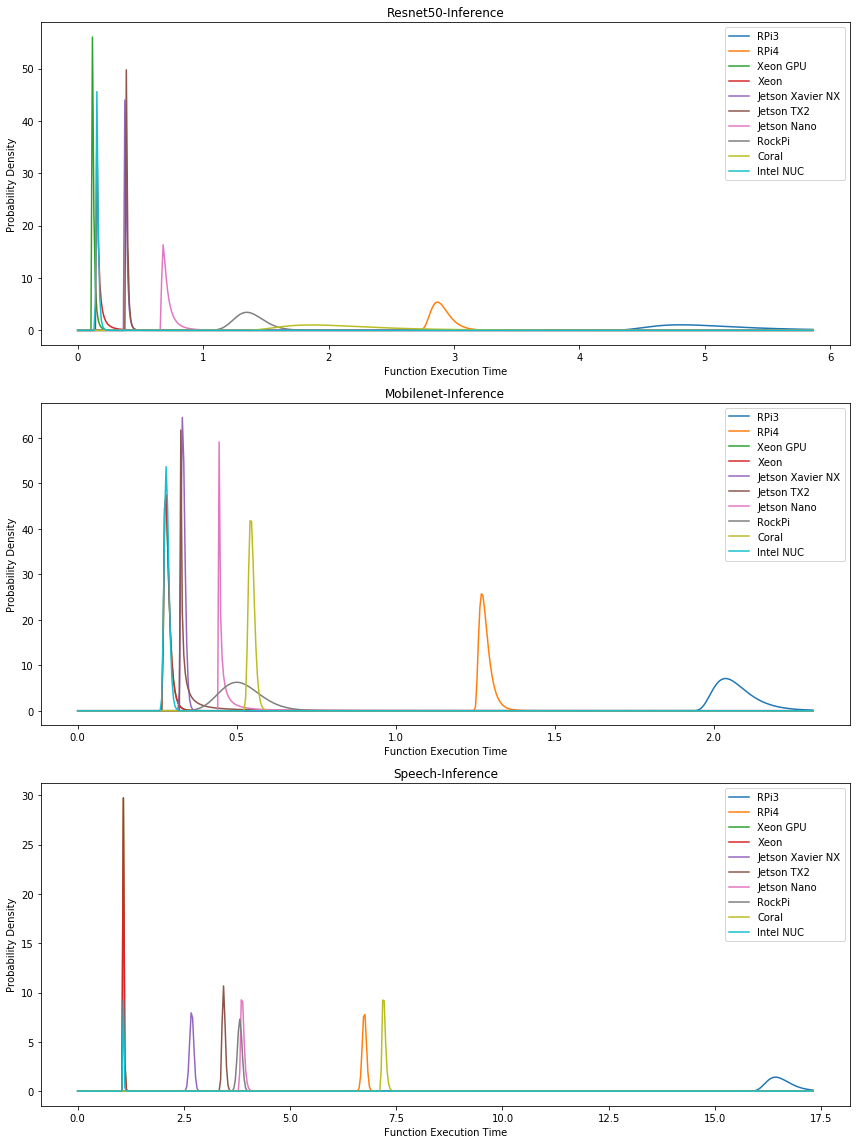
\includegraphics[width=\linewidth]{graphics/graphs/devices_fets.png}
    \caption{Probability density functions of the \glspl{fet} of the different devices we simulate}
    \label{fig:devices_fets}
\end{figure}

Figure \ref{fig:devices_fets}
shows the \gls{fet} distributions for these functions on the hardware outlined in Table \ref{tab:ether_devices}.

Because FaaS-Sim originally only supported response time evaluations due to \gls{fet}, we extend it to also include the network time incurred from request transfers.
To enable this functionality, we introduce the notion of clients explicitly.
They are represented via nodes in the underlying network topology, just like the serverless cluster's nodes are.
Each request is dispatched from a client, sent to the nearest running load balancer instance, on to the function instance the load balancer selects, and back the same way.

The load pattern clients exhibit in FaaS-Sim can be fully controlled.
Generally, clients follow a predefined request pattern, either individually or globally, but absolutely any pattern required can be implemented.
This allows the simulation of differently active clients, differently active regions, and request patterns that change depending on system parameters.

To extract data for later analysis, FaaS-Sim features fine-grained and extensible trace-logging of all requests and system events.
\section{Network Simulation and Topologies}
Because this work places a particular emphasis on network optimization, the network simulation component of FaaS-Sim is of particular relevancy to us.
Under the hood, FaaS-Sim relies on Ether\cite{rausch-ether} for its networking.

Aside from vast option for customization, Ether supports a number of networking primitives that allow us to easily create a range of topologies.
In Ether's model, resources are usually, but not necessarily, grouped together in a cell.
The most important ones for our case are the \textit{LAN Cell} and the \textit{Shared Link Cell}.
The LAN Cell represents a set of compute nodes which are interconnected with each other in the way a LAN typically is, which means bandwidth is high, latency low, and variance small.\\
Contrary to that Shared Link Cells are more typical of what we might expect in an IoT scenario. 
It represents multiple nodes, which, as the name suggests, share a network connection between them.
This can, for example, be used to represent a number of edge devices which are grouped together into a small compute box and share a mobile internet connection for wider connectivity.

The networking simulation in Ether is based around the \textit{Link} object\cite{rausch-ether}, which represents a connection between nodes.
A mobile network connection, for example, would be considered a Link.
As Links represent connections, they also have a set bandwidth and latency.
To more accurately simulate how networks behave in real life, the latency of a link is not defined as a fixed number, but as a random distribution which gets sampled during simulation.

% decided to do a textual representation, as it was more useful
% this is just a placeholder in case I change my mind

To simulate network transfers Ether uses a flow-based simulation.
The transfer of a request from one node to another is considered a flow.
For each flow two steps are simulated: TCP connection establishment, and data transfer.
TCP connection establishment is assumed to be equal to $ 3 \times \text{latency}$ of the route the flow takes, based on the three-way SYN, SYN-ACK, ACK handshake of the TCP protocol.\\
The data transfer is where the flow simulation component is used.
Each flow consists of a number of hops, connected by links.
Each of these links has a set latency, bandwidth, and potentially a number of other flows currently being transferred.
To calculate how long data transfer takes, we first determine the bandwidth.
The bandwidth is determined by the minimum bandwidth available from any of the flow's links.
What exactly this is depends on the general bandwidth of the link in question, and by how many flows have to share this available bandwidth.
Once the bandwidth of the flow is determined we can simply calculate how long data transfer will take, given a request of known size.
To preserve the impact different flows have on each other, once a flow is added to the system, or once a flow is completed and thus removed, every link of the flow is updated and potentially recalculates the bandwidth of other running flows.
Other flows might be unaffected, but may also see and increase or decrease in available bandwidth depending on whether there are now more or fewer flows competing.
If flows are competing for bandwidth, they are all treated with equal priority, and share equally in the available bandwidth.


The topologies we use for our evaluations are based on the concept of smart cities\cite{suSmartCityApplications2011}.
In this context we assume there may or may not be a central point in the city which provides a high amount of computational capability, i.e. a data center, and that the majority of computational capability will be interspersed throughout the city alongside with the clients.

For these edge-located resources we assume that two major types exist: \textit{Smart Poles} and \textit{\gls{ran} Towers}.
We consider \gls{ran} Towers to be any type of LTE or 5G mobile base station, which in our smart city scenario would additionally be equipped with edge computing capability.
The Smart Poles we consider to be a functionally similar, though comparatively smaller device, much like the Huawei PoleStar\cite{huaweiPolestar}, which is also equipped with computational capability, albeit less of it, and providing a connection to the wider network.
We assume that these Smart Poles would be spread out throughout the city like sensor nodes in the Array of Things\cite{catlettArrayThingsScientific2017a}, a real world edge computing and smart city sensing deployment.
In terms of latency and bandwidth we assume latency to Smart Pole devices to be in the same ballpark as WiFi connections, while \gls{ran} Tower connections are in line with what one would typically expect of LTE or 5G connections respectively.
In keeping with our methodology of informing simulation values with real world measurements where possible, we used the research conducted by Braud et al.\cite{braudMulticarrierMeasurementStudy2019} and Nikravesh et al.\cite{nikraveshMobileNetworkPerformance2014a} on real world LTE network characteristics to inform our parametrization of these connections.
We also assume that truly low latency connections for client devices are only provided by physically near access points such as the aforementioned Smart Pole devices, as research on wireless network technology indicates that there is a fundamental tradeoff between bandwidth, latency, and reliability\cite{soretFundamentalTradeoffsReliability2014}.

\begin{figure}
    \centering
    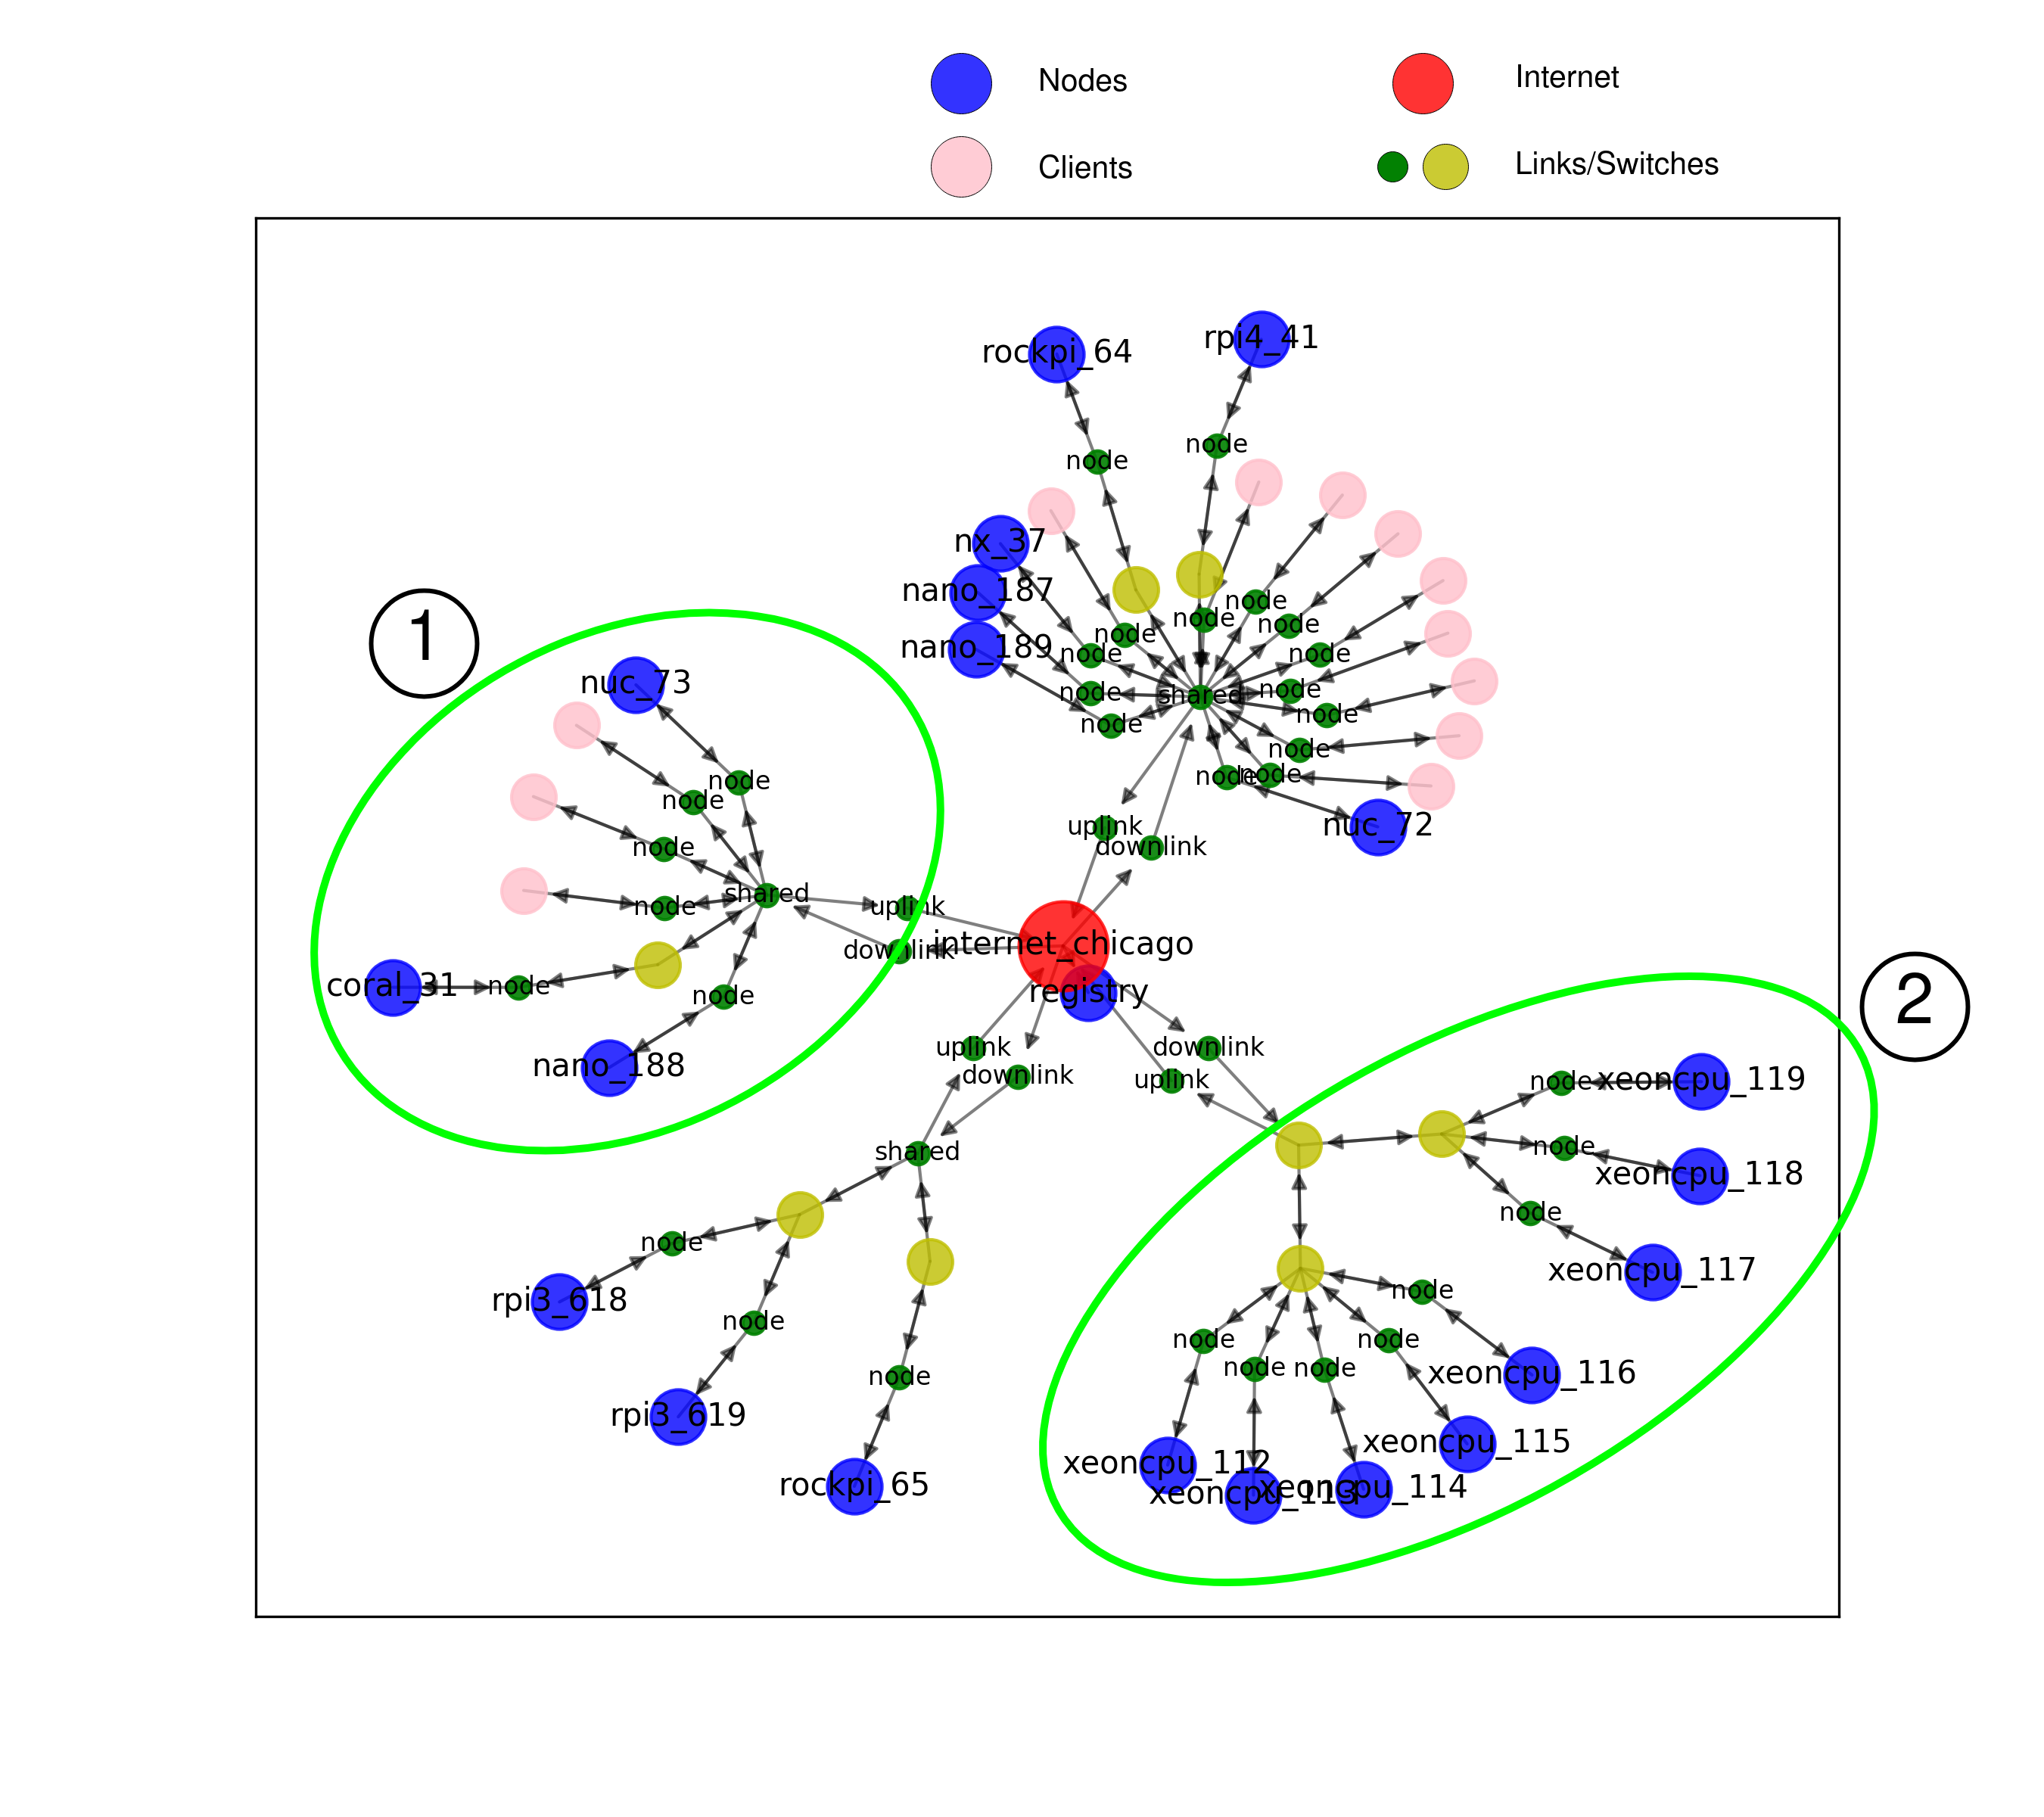
\includegraphics[width=\linewidth]{graphics/diagrams/tiny_topo.png}
    \caption{Simplified network topology of a single smart city. Centered around the internet backbone uplink (red), 1) shows edge devices co-located with client devices. 2) shows a small cloud data center or cloudlet. Note the lack of clients directly connected to the cloudlet.}
    \label{fig:tiny_topo}
\end{figure}

Finally, Figure \ref{fig:tiny_topo} shows a simplified visualization of how one of our smart city topologies is structured.
Note that latency cannot be read from this visualization and that distances between nodes on the visualization do not correspond to network distances whatsoever.
The wider internet, presented as a red circle, is how communication to areas not deemed within the city, or general web-services such as container registries would be routed.
Also note that we only represent logical network links and connections in our topologies, which means that while in truth there might be tens of network hops between an edge node and the wider internet (e.g. through the nearest backbone uplink), for simulation performance reasons we do not include these in our model.
% 1 page
\section{Using Empirical Data in Simulations}
As already described FaaS-Sim\cite{faas-sim-github}, the serverless simulator we use, is a trace-driven simulator\cite{thomas-thesis}, meaning that it relies on measurements of real world data to make its results more representative.
The types of empirical data that can be used to improve simulation accuracy are very broad, but are typically limited to those that actually affect the metrics one is interested in measuring.
Usually this includes the memory consumption, CPU utilization, network utilization and storage size of different software components present in the system.
It can, however, also include more specific metrics such as deployment, staring, stopping and teardown times of container in a Kubernetes cluster\cite{skippy}.

Similar to how Raith et al. extended FaaS-Sim to include traces of real function executions to better represent \glspl{fet} \cite{philipp-da}, we perform experiments to inform how load balancers are modelled within the system.
Since in current serverless frameworks ingress-points, which is equivalent to a load balancer in our case, are considered as just another service, they compete with function replicas for resources.
As a result the resource usage of typical application level load balancers is an important metric for us to capture and integrate into the serverless simulator.

For our empirical evaluations we use a real Kubernetes cluster that features a variety of heterogeneous nodes.
Since we deal with edge computing applications, and resource heterogeneity is a core challenge of edge computing\cite{shiEdgeComputingVisionChallenges2016}, having a range of different nodes to evaluate performance on is critical to account for variance incurred by the use of different types of devices.
We also make use of and extend galileo\cite{galileo-github}\cite{operating-energy-aware-galileo}, a framework built for distributed load testing, as it allows us to easily define request patterns and loads that then get executed.
By using this we can go beyond measurements of baseline resource consumption and examine the relationship between the request load of a service and its performance and resource consumption profile.
To gather performance data of individual containers in a Kubernetes cluster, galileo relies on and integrates with telemd\cite{telemd-github}.
Telemd is a daemon application that can gather a number of system metrics at specified intervals, including CPU utilization, memory consumption, disk I/O, and network transfers.


% what do I actually want to say?
% empirical experiments important to inform real world data
% need to be aligned with the hardware simulated e.g. arm devices, x86, etc. etc.
% this needs to be measured somehow -> galileo
%
%
% 1-2 pages
\section{Captured Metrics}
There is a significant number of metrics that could be captured using such a simulation. With FaaS-Sim we capture traces of the requests being sent, and major system events.
The major system events are the addition or removal of deployments, as well as all scaling and scheduling decisions with respect to functions and load balancers.
For requests our traces provide the following information: \gls{trt}, \gls{fet}, waiting time, request client, load balancer instance, function instance, and the network times between client, load balancer and function instance.
The waiting time refers to the elapsed between a request having been received by a function instance, and the request being processed.
Waiting times occur if a node receives requests faster than it can process them.
In terms of resource usage, the resources reserved by the simulated Kubernetes pods, which correspond to the requirements defined in Kubernetes deployment manifests, are also recorded.
Note that this does not necessarily correspond to actual resource usage.
Because these reserved resource metrics are used for Kubernetes' scheduling decisions, we believe they are still worth being captured.

In keeping with the set of potential metrics outlined by Aslanpour, Gill and Toosi\cite{aslanpourPerformanceEvaluationMetrics2020a}, we pay particular attention to response times, potential \gls{sla} levels and oscillation mitigation.
We also introduce more qualitative metrics, related to our particular evaluation scenario, such as the share of requests being routed outside of the city or network region they originate in.